% Provenance (never printed): see sources/outline_sources.md (Year 1: elastic rebound and the
% seismic cycle; seismic moment and magnitudes; focal mechanisms; geodetic measurement of
% active deformation; the Gutenberg--Richter law). Exercise and problem values in the Book 3
% scratch calculator calc/ch18.py; figure data from figdata/bachelor-1/gutenberg_richter.py,
% beachballs.py and interseismic.py. Focus, epicentre, magnitude, intensity and seismometer
% are owned by Book 1 g7 (magnitude re-founded here as the moment magnitude); P and S waves by
% Book 2 g11; fault types and rake by ch. 17; stress, Coulomb and the seismogenic layer by
% ch. 16; the shear modulus by physics. Radar interferometry and the stereographic projection
% belong to later volumes (told, not defined).
\chapter{The Earthquake Source}\label{ch:b1:earthquake-source}

% ledger: pp1515:1906, reid:1910
On the morning of 18 April 1906, the ground north and south of San Francisco
broke along a line more than four hundred kilometres long. Roads, fences and
rows of trees that crossed the line were cut, and the two halves of each were
found metres apart, the western half always displaced to the north. Surveyors
had measured the positions of landmarks in the region during the previous
half-century, and when the landmarks were measured again the
comparison showed something stranger than the break itself: the ground had
been bending, slowly and smoothly, for decades before the earthquake, and the
earthquake had let it spring back. This chapter follows an earthquake from
the slow loading of a fault to the few minutes in which it slips, and reads
the slip back from the waves and from the ground: how large it was, in which
direction it moved, how fast the next one is being prepared, and how often
earthquakes of each size come.

\begin{recall}
The focus of an earthquake is the point where the rupture starts, its
epicentre the point of the surface above it; the magnitude measures the size
of an earthquake, the intensity the shaking at a place; a seismometer records
the ground's motion as a seismogram (Book~1, grade~7). The P wave, a
compressional wave, arrives first and the S wave, a shear wave, after it
(Book~2, grade~11). A fault has a \omterm{def:b1:faults-folds-fabrics:fault-elements}{hanging wall} and a \omterm{def:b1:faults-folds-fabrics:fault-elements}{footwall}; the \omterm{def:b1:faults-folds-fabrics:fault-elements}{slip vector}
is the displacement of the \omterm{def:b1:faults-folds-fabrics:fault-elements}{hanging wall} relative to the \omterm{def:b1:faults-folds-fabrics:fault-elements}{footwall}, its \omterm{def:b1:faults-folds-fabrics:fault-elements}{rake}
$r$ is measured on the fault plane from the \omterm{def:b1:geological-maps:attitude}{strike}, and the \omterm{def:b1:faults-folds-fabrics:fault-elements}{rake} names the
fault: about \ang{90} reverse, about \ang{-90} normal, about 0 \omterm{def:b1:faults-folds-fabrics:fault-types}{sinistral}, about
\ang{180} \omterm{def:b1:faults-folds-fabrics:fault-types}{dextral} (\cref{ch:b1:faults-folds-fabrics}). An elastic solid
returns to its shape when the stress is removed; the shear modulus $\mu$
relates a shear stress to the \omterm{def:b1:stress-strain-rheology:strain}{shear strain} it produces (physics); faults slip
when the shear stress reaches their frictional strength, and earthquakes
start in the brittle upper part of the \omterm{def:b1:layered-earth:layers}{crust}, the \omterm{def:b1:stress-strain-rheology:strength-envelope}{seismogenic layer}
(\cref{ch:b1:stress-strain-rheology}). Permanent satellite-positioning
stations, whose daily positions over years give the velocity of the ground
where they stand, measure the motions of plates (\cref{ch:b1:plate-kinematics}).
\end{recall}

\section{Elastic rebound and the seismic cycle}\label{sec:b1:earthquake-source:cycle}

Two plates that slide past each other at a steady rate do not, in general,
slide steadily along the fault between them. Friction holds the fault locked
while the plates keep moving far from it, so that the rocks on either side are
bent like a spring. When the shear stress on the fault reaches its strength,
the fault slips in a few seconds or minutes, and the bent rocks snap back.

\begin{definition}[Elastic rebound, seismic cycle, recurrence interval]\label{def:b1:earthquake-source:seismic-cycle}
\emph{Elastic rebound}\index{elastic rebound} is the sudden return toward
their unstrained shape of the rocks on either side of a fault, when the fault,
locked while they were strained, slips in an earthquake; the elastic energy
stored in them is released, partly as seismic waves. The \emph{seismic
cycle}\index{seismic cycle} of a fault segment is the repeated sequence of a
long interseismic stage, during which the segment is locked and the strain
accumulates around it, a coseismic stage, the earthquake, during which it
slips, and a postseismic stage, of months to decades, during which the
surroundings adjust to the new state. The \emph{recurrence
interval}\index{recurrence interval} of a segment is the time between two
successive large earthquakes on it.
\end{definition}
% ledger: usgs:gloss-rebound, reid:1910, usgs:pp1515-thatcher

\begin{omfigure}
\begin{tikzpicture}[>={Stealth[length=5pt]}, font=\small]
% map view of a fence across a locked dextral strike-slip fault (north up): (a) built straight;
% (b) after decades of loading, bent with the interseismic profile v(x) = -(s/pi) arctan(x/D)
% (dextral: the east side moves south); (c) after the earthquake, straight again on each side and
% offset by s at the fault. Panel 3.4 cm wide (x from -1.7 to 1.7 cm), D = 0.35 cm, s = 0.9 cm.
\def\s{0.9}\def\Dl{0.35}
\foreach \k/\t in {0/{(a) the fence is built}, 1/{(b) decades of loading}, 2/{(c) after the earthquake}} {
  \begin{scope}[xshift=\k*4.6cm]
    \fill[omLithSand!25] (-1.7,-1.6) rectangle (1.7,1.6);
    \draw[black!50, line width=0.4pt] (-1.7,-1.6) rectangle (1.7,1.6);
    \draw[fault, line width=1.1pt] (0,-1.6) -- (0,1.6);
    \node[anchor=north, align=center, font=\scriptsize] at (0,-1.7) {\t};
    % far-field motion of the two blocks, relative to the fault
    \draw[->, omThm, line width=0.8pt] (-1.35,-1.25) -- (-1.35,-0.45);
    \draw[->, omThm, line width=0.8pt] (1.35,1.25) -- (1.35,0.45);
    \ifnum\k=0
      \draw[line width=1.2pt, omDef] (-1.7,0) -- (1.7,0);
    \fi
    \ifnum\k=1
      \draw[line width=1.2pt, omDef] plot[domain=-1.7:1.7, samples=81, variable=\x] (\x, {-\s/pi*atan(\x/\Dl)*pi/180});
      \draw[black!45, dashed, line width=0.4pt] (-1.7,0) -- (1.7,0);
    \fi
    \ifnum\k=2
      \draw[line width=1.2pt, omDef] (-1.7,{\s/2}) -- (0,{\s/2});
      \draw[line width=1.2pt, omDef] (0,{-\s/2}) -- (1.7,{-\s/2});
      \draw[black!45, dashed, line width=0.4pt] (-1.7,0) -- (1.7,0);
      \draw[<->, line width=0.5pt] (0.18,{\s/2}) -- (0.18,{-\s/2});
      \node[anchor=west, font=\scriptsize] at (0.2,0.12) {slip};
    \fi
  \end{scope}
}
\node[anchor=south, font=\scriptsize] at (0,1.62) {fault};
\draw[->, line width=0.5pt] (-1.5,0.75) -- (-1.5,1.15) node[above, font=\scriptsize, inner sep=1pt] {N};
\end{tikzpicture}
\par\smallskip{\small \omterm{def:b1:earthquake-source:seismic-cycle}{Elastic rebound} seen from above, on a fence (blue)
built straight across a locked \omterm{def:b1:faults-folds-fabrics:fault-types}{dextral} fault. Red arrows: the motion of the
two blocks far from the fault, relative to it. (b) While the fault is locked,
the far ground moves and the fence bends, along the curve of the
interseismic profile of \cref{sec:b1:earthquake-source:geodesy}. (c) The
earthquake releases the bending: each half of the fence is straight again, and
the two halves are offset at the fault by the slip. The bending is
exaggerated: a real fence bends by a few metres over tens of kilometres.}
\label{fig:b1:earthquake-source:rebound}
\end{omfigure}

If the fault is locked between earthquakes and each earthquake undoes the
slip the plates have accumulated since the last one, the plate motion sets the
pace of the cycle.

\begin{proposition}[Recurrence from the slip rate]\label{prop:b1:earthquake-source:recurrence}
Let a fault segment be loaded at the long-term slip rate $\dot s$, be locked
between earthquakes, and slip by the same amount $D$ in each earthquake. Then
the \omterm{def:b1:earthquake-source:seismic-cycle}{recurrence interval} of its earthquakes is
\[
  T = \frac{D}{\dot s} .
\]
If only the fraction $c$ of the slip rate is locked, the rest slipping
steadily without earthquakes, $T = D/(c\,\dot s)$.
\end{proposition}

\begin{proof}
Over a long time $t$, the two sides of the fault move by $\dot s\,t$ relative to
each other. Far from the fault the ground moves steadily, so on the fault
itself the same displacement must be made up, here by earthquakes alone: if
$N$ earthquakes happened in the time $t$, then $N D = \dot s\,t$ up to the
slip of one earthquake, and $t/N \to D/\dot s$. With the fraction $1-c$ of the
slip made by steady sliding, the earthquakes make up $c\,\dot s\,t$ and
$t/N \to D/(c\,\dot s)$.
\end{proof}

With values typical of the San Andreas fault, a slip of \qty{4}{m} in each great
earthquake and a slip rate of \qty{20}{mm.yr^{-1}}, the \omterm{def:b1:earthquake-source:seismic-cycle}{recurrence interval} is
\qty{200}{yr}. At Wallace Creek, in central California, a stream channel cut
across the fault has been offset by \qty{128}{m} in the \num{3587} years since
it was incised, an average of \qty{36}{mm.yr^{-1}}, close to the rate of about
\qty{34}{mm.yr^{-1}} measured on other offsets there; the last great earthquake
on that stretch, in 1857, slipped by nearly \qty{10}{m}, which at this rate takes
about three centuries to accumulate.
% ledger: usgs:pp1515-thatcher, usgs:pp1515-wallace, commons:wallace-creek

\begin{omfigure}
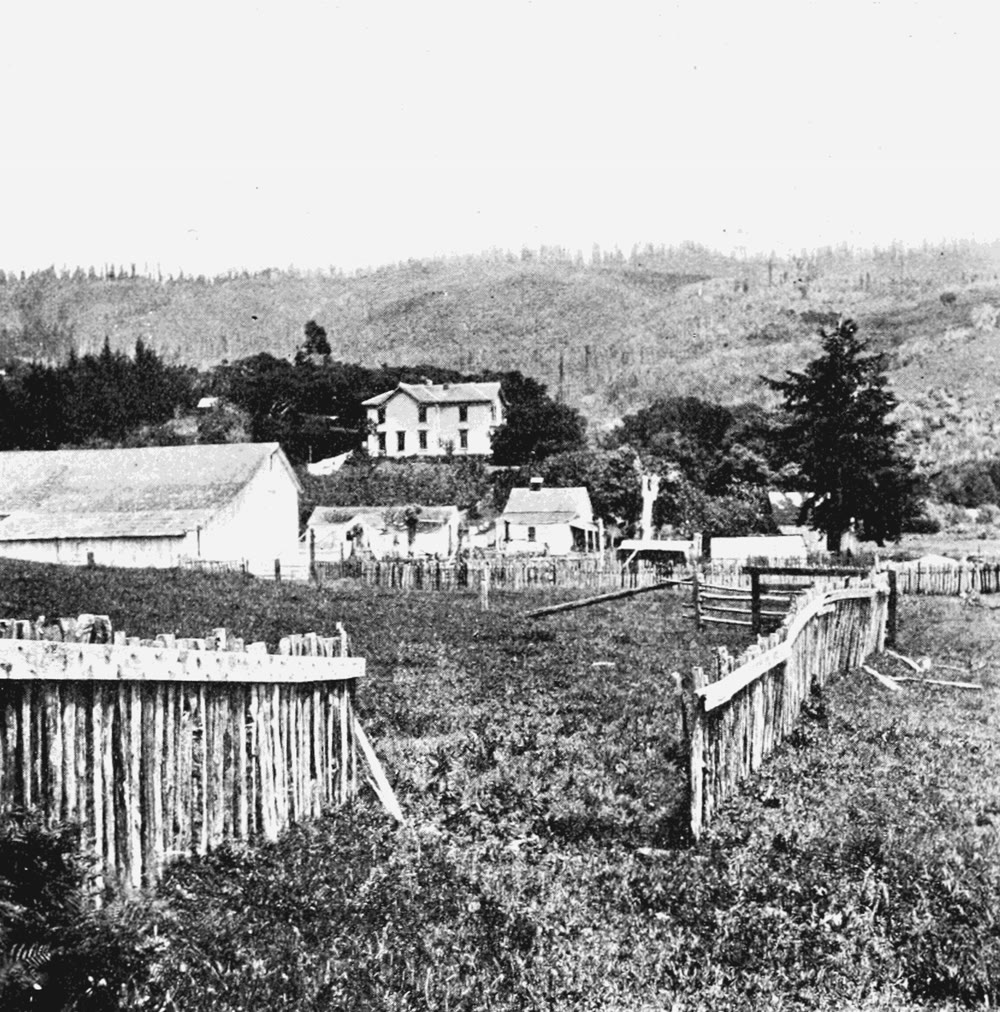
\includegraphics[height=5.6cm]{images/book3/b1-fence-1906.jpg}\hfill
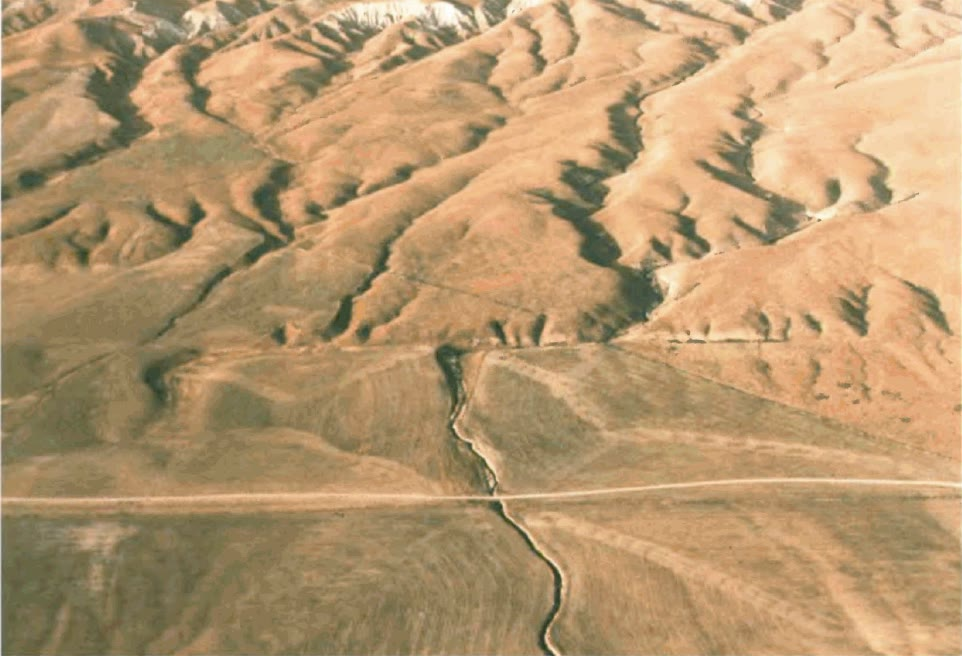
\includegraphics[height=5.6cm]{images/book3/b1-wallace-creek.jpg}
\par\smallskip{\small Left: fences in farmland of Marin County, north of San
Francisco, crossed by the 1906 rupture, published the same year as ``land
separated by the earthquake fault''. Photograph from \emph{Popular Science
Monthly}, vol.~69 (1906), public domain. Right: Wallace Creek, Carrizo Plain,
seen from the air: the stream comes down from the hills (top), and where it
crosses the San Andreas fault, at the foot of the hills, its channel jogs
sideways by \qty{130}{m}, the offset accumulated over thousands of years of
earthquakes. Photograph:
R.~E.~Wallace, U.S. Geological Survey, public domain. Both from Wikimedia
Commons.}
\label{fig:b1:earthquake-source:offsets}
\end{omfigure}
% ledger: commons:psm-fence, commons:wallace-creek

The proposition gives an average, not a timetable. Near Parkfield, on the
same fault, an earthquake of magnitude about 6 in 1857 was followed by five
more, much alike, on the same stretch of some \qty{30}{km}, at intervals of
nearly 22 years up to 1966; the next was expected before 1993, and came in
2004, with a \omterm{def:b1:earthquake-source:mw}{moment magnitude} of 6.0 and without any clear warning sign. The
strength of a fault, the slip of each earthquake and the loading by its
neighbours all vary from one cycle to the next, and the \omterm{def:b1:earthquake-source:seismic-cycle}{seismic cycle} is
better described by a mean \omterm{def:b1:earthquake-source:seismic-cycle}{recurrence interval} and a spread about it than by
a period.
% ledger: pp1515:parkfield, bl85:parkfield, usgs:hist-mw, bakun:2005

Some fault segments do not lock at all. Between Parkfield and San Juan
Bautista, the central section of the San Andreas fault creeps: steady slip on
the fault takes up nearly all the motion of the plates, and little if any
strain builds up on either side, so that this section has no great
earthquakes; the great rupture of 1857 started at its southern end and that of
1906 stopped at its northern one. A fault that creeps over part of its area is
locked only in part, which is the coefficient $c$ of the proposition.
% ledger: pp1515:creep, pp1515:1906

\begin{inthefield}[Reading past earthquakes in a trench]
Instruments have recorded earthquakes for little more than a century, much
less than one cycle of most faults. Palaeoseismologists extend the record by
reading the ground. A trench a few metres deep is dug across an active fault
where layers of sediment have been laid down continuously, in a marsh, a lake
or a small alluvial fan. On its walls, each earthquake shows as layers cut and
offset by the fault and covered, unbroken, by younger ones; as a scarp buried
by later deposits; as sand that liquefied and rose through cracks to spread
over the surface of the time. Peat or plant remains in the layers just below
and just above each break are dated by radiocarbon, and so bracket the date of
each earthquake: one marsh on the San Andreas fault holds the record of twelve.
Along coasts, sheets of sand laid down by tsunamis and marshes that sank
suddenly by a metre or so, buried under tidal mud, record the great subduction
earthquakes. On the San Andreas fault, most of the slip of historical times
came with earthquakes of magnitude 6 or more.
\end{inthefield}
% ledger: pp1515:pallett, atwater:1987

\begin{history}[Harry Fielding Reid and elastic rebound]
Harry Fielding Reid, an American physicist, was a member of the state
commission that studied the 1906 earthquake. Comparing the positions of
points surveyed in 1851--1865, in 1874--1892 and after the earthquake, he
found that distant points on the two sides of the San Andreas fault had moved
by about \qty{3.2}{m} relative to each other since the first survey, a little
more than half the slip of about \qty{6}{m} on the fault: half a century before
the earthquake, the strain that broke the fault was already half built. Only
elastic forces could have moved the ground so suddenly, and he called the
sudden return \omterm{def:b1:earthquake-source:seismic-cycle}{elastic rebound}. He published it in the second volume of the
commission's report, in 1910; it is still the principal model of the
earthquake cycle. Satellite positioning has since measured the bending he
could only infer.
\end{history}
% ledger: reid:1910, pp1515:1906

\section{Seismic moment and magnitude}\label{sec:b1:earthquake-source:moment}

The size of an earthquake is the amount of slip it made, over the area of
fault that slipped, weighted by how stiff the rocks are.

\begin{definition}[Seismic moment]\label{def:b1:earthquake-source:moment}
Let an earthquake slip by the average amount $D$ over a rupture of area $A$,
in rocks of shear modulus $\mu$ (the letter also names a coefficient of friction,
in \cref{ch:b1:stress-strain-rheology}; the context tells which). Its \emph{seismic moment}\index{seismic
moment} is
\[
  M_0 = \mu A D ,
\]
in newton metres.
\end{definition}
% ledger: usgs:gloss-moment

The unit is that of a torque. A slip on a fault sends out the same waves as two
pairs of opposed forces, two couples, applied at the focus, and the \omterm{def:b1:earthquake-source:moment}{seismic
moment} is the moment of each couple (this equivalence, the double couple, is
proved in the Year~3 volume). The moment has the dimensions of an energy, but
it is not one: the energy radiated as waves is a small fraction of it. For the
rocks of the \omterm{def:b1:layered-earth:layers}{crust}, $\mu$ is taken as \qty{30}{GPa}.
% ledger: kanamori:1977, sk:mu-locking

The moment is computed today from the long-period waves recorded around the
world. For the Tohoku earthquake of 11 March 2011, the preferred solution of
the U.S. Geological Survey gives $M_0 = \qty{5.59e22}{N.m}$. The fault slipped
over an area about \qty{400}{km} long and \qty{150}{km} wide; the definition
then gives the average slip
\[
  D = \frac{M_0}{\mu A}
    = \frac{\num{5.59e22}}{\num{3e10}\times\num{4e5}\times\num{1.5e5}}
    \approx \qty{31}{m} ,
\]
and models of the rupture find up to \qtyrange{50}{60}{m} in its most
displaced part.
% ledger: usgs:tohoku-mt, usgs:tohoku-summary

The magnitude of Book~1 was worked out from the amplitude of the waves on a
seismogram. Such magnitudes measure the waves of one period; once a rupture is
much longer than their wavelength, a few to some fifty kilometres, the
amplitude stops growing with its size, and the magnitude saturates. The
body-wave magnitude saturates near 6.5, the surface-wave magnitude near 8.3.
In 2011, the first tsunami warning for Tohoku was based on a magnitude of this
kind, which falls short for earthquakes of magnitude 8 or more, and it
underestimated the waves. The moment does not saturate, and the magnitude is
now defined from it.
% ledger: kanamori:1977, usgs:magtypes, jma:warning

\begin{definition}[Moment magnitude]\label{def:b1:earthquake-source:mw}
The \emph{moment magnitude}\index{moment magnitude} of an earthquake of
\omterm{def:b1:earthquake-source:moment}{seismic moment} $M_0$, in newton metres, is
\[
  M_w = \tfrac23\left(\log_{10} M_0 - 9.1\right) .
\]
\end{definition}
% ledger: usgs:magtypes

Thomas Hanks and Hiroo Kanamori defined the scale in 1979, with the constant
9.05 in place of 9.1, a difference of 0.03 in $M_w$; the constants were chosen
to match the older magnitudes where those do not saturate. The magnitude of
Book~1 is, for large earthquakes, this number: for Tohoku,
$M_w = \tfrac23(\log_{10}\num{5.59e22} - 9.1) = \tfrac23(22.75 - 9.1) = 9.1$;
the great Chilean earthquake of 1960 and the Alaskan earthquake of 1964 have
\omterm{def:b1:earthquake-source:mw}{moment magnitudes} of 9.5 and 9.2, sizes that the older magnitudes could not
show.
% ledger: hk:1979, kanamori:1977, usgs:hist-mw, usgs:tohoku-mt

\begin{proposition}[One unit of magnitude]\label{prop:b1:earthquake-source:moment-steps}
The \omterm{def:b1:earthquake-source:moment}{seismic moment} is $M_0 = 10^{1.5 M_w + 9.1}$ newton metres. One unit of
\omterm{def:b1:earthquake-source:mw}{moment magnitude} multiplies it by $10^{1.5} \approx 31.6$, two units by
$1000$. If the energy radiated is a fixed fraction of the moment, it grows in
the same ratio.
\end{proposition}

\begin{proof}
Solving the definition for $M_0$ gives $\log_{10} M_0 = 1.5 M_w + 9.1$,
and for two earthquakes
\[
  \log_{10}\frac{M_0'}{M_0} = 1.5\,(M_w' - M_w) ,
\]
which is $1.5$ for one unit and $3$ for two. If the radiated energy is $E_s = k M_0$ with the same $k$
for both, $E_s'/E_s = M_0'/M_0$.
\end{proof}

Kanamori's approximation, $E_s \approx M_0/(2\times10^4)$ (admitted), is the
assumption of the last sentence; the factor of about 32 in energy per unit of
magnitude, met in Book~1, is this proposition. Since $M_0 = \mu A D$ and the
slip of an earthquake grows with the size of its rupture, a large magnitude
needs a large fault. The 1906 rupture, about \qty{430}{km} long, broke the
\omterm{def:b1:stress-strain-rheology:strength-envelope}{seismogenic layer} to about \qty{15}{km} with an average slip of a few metres:
with $D = \qty{4}{m}$, $M_0 = \num{3e10}\times\num{4.3e5}\times\num{1.5e4}
\times 4 = \qty{7.7e20}{N.m}$ and $M_w = 7.9$, the magnitude of the catalogue.
A magnitude of 9 needs a rupture of hundreds of kilometres in length and more
than a hundred in width, which only the gently dipping interfaces of
subduction zones offer.
% ledger: kanamori:1977, pp1515:1906, usgs:hist-mw, usgs:pp1515-thatcher

\section{Focal mechanisms}\label{sec:b1:earthquake-source:focal}

The P wave is the first to reach a seismometer. Its \omterm{def:b1:earthquake-source:focal-mechanism}{first motion}, the first
swing of the vertical record, is up where the wave arrives as a push, the
ground compressed and thrown away from the source, and down where it arrives
as a pull. Around an earthquake, pushes and pulls are arranged in a pattern
that gives the orientation of the fault and the direction of slip.

\begin{proposition}[The sign of the first motion]\label{prop:b1:earthquake-source:first-motion}
Let a fault of upward normal $\mathbf n$ slip by the unit vector $\mathbf d$
(the slip of the \omterm{def:b1:faults-folds-fabrics:fault-elements}{hanging wall} relative to the \omterm{def:b1:faults-folds-fabrics:fault-elements}{footwall}). The P wave that leaves
the focus in the unit direction $\mathbf x$ arrives as a push if
$(\mathbf n\cdot\mathbf x)(\mathbf d\cdot\mathbf x) > 0$ and as a pull if
$(\mathbf n\cdot\mathbf x)(\mathbf d\cdot\mathbf x) < 0$. The pushes and the
pulls thus fill four quadrants, separated by the fault plane
($\mathbf n\cdot\mathbf x = 0$) and by the plane perpendicular to the slip
($\mathbf d\cdot\mathbf x = 0$).
\end{proposition}

\begin{proof}
A direction with $\mathbf n\cdot\mathbf x > 0$ points into the \omterm{def:b1:faults-folds-fabrics:fault-elements}{hanging wall},
which moves by $\mathbf d$ relative to the \omterm{def:b1:faults-folds-fabrics:fault-elements}{footwall}: the rock ahead of it,
where $\mathbf d\cdot\mathbf x > 0$, is compressed, and the rock behind it,
where $\mathbf d\cdot\mathbf x < 0$, is pulled. A direction with
$\mathbf n\cdot\mathbf x < 0$ points into the \omterm{def:b1:faults-folds-fabrics:fault-elements}{footwall}, which moves by
$-\mathbf d$ relative to the \omterm{def:b1:faults-folds-fabrics:fault-elements}{hanging wall}, so the signs are reversed. In each
case the \omterm{def:b1:earthquake-source:focal-mechanism}{first motion} has the sign of $(\mathbf n\cdot\mathbf x)(\mathbf
d\cdot\mathbf x)$.
\end{proof}

The argument gives the sign only. The amplitude of the \omterm{def:b1:earthquake-source:focal-mechanism}{first motion}, which is
proportional to $2(\mathbf n\cdot\mathbf x)(\mathbf d\cdot\mathbf x)$ and so
largest at \ang{45} from both planes and zero on them, is admitted here
(Year~3 volume).

\begin{omfigure}
\begin{tikzpicture}[>={Stealth[length=5pt]}, font=\small, scale=0.95]
% map view around a vertical dextral fault striking north, the focus at the origin, rays leaving
% horizontally: pushes where (n.x)(d.x) > 0, i.e. in the NW and SE quadrants (beachballs.py,
% first_motion(0, 90, 180, x)). Stations at 20 azimuths on a circle of radius 2.3.
\fill[omThm!22] (0,0) -- (0,2.8) arc[start angle=90, end angle=180, radius=2.8] -- cycle;
\fill[omThm!22] (0,0) -- (0,-2.8) arc[start angle=270, end angle=360, radius=2.8] -- cycle;
\draw[black!40, line width=0.4pt] (0,0) circle[radius=2.8];
\draw[fault, line width=1.3pt] (0,-3.1) -- (0,3.1) node[above, font=\scriptsize] {fault (nodal plane)};
\draw[black, dashed, line width=0.7pt] (-3.1,0) -- (3.1,0) node[right, font=\scriptsize, align=left] {auxiliary\\ plane};
% slip: the west block moves north, the east block south
\draw[->, line width=1pt] (-0.3,-0.8) -- (-0.3,0.8);
\draw[->, line width=1pt] (0.3,0.8) -- (0.3,-0.8);
% stations
\foreach \a in {9,27,...,351} {
  \pgfmathsetmacro{\fm}{-sin(\a)*cos(\a)}  % (n.x)(d.x) with n = east, d = south, x = (sin a, cos a)
  \pgfmathparse{\fm>0 ? 1 : 0}
  \ifnum\pgfmathresult=1
    \fill[black] ({2.3*sin(\a)},{2.3*cos(\a)}) circle[radius=0.11];
  \else
    \draw[black, fill=white, line width=0.6pt] ({2.3*sin(\a)},{2.3*cos(\a)}) circle[radius=0.11];
  \fi
}
% P and T axes
\draw[<-, omProp, line width=1.1pt] ({0.7*sin(45)},{0.7*cos(45)}) -- ({1.6*sin(45)},{1.6*cos(45)}) node[above right, font=\scriptsize, inner sep=1pt] {P};
\draw[<-, omProp, line width=1.1pt] ({0.7*sin(225)},{0.7*cos(225)}) -- ({1.6*sin(225)},{1.6*cos(225)});
\draw[->, omProp, line width=1.1pt] ({0.7*sin(315)},{0.7*cos(315)}) -- ({1.6*sin(315)},{1.6*cos(315)}) node[above left, font=\scriptsize, inner sep=1pt] {T};
\draw[->, omProp, line width=1.1pt] ({0.7*sin(135)},{0.7*cos(135)}) -- ({1.6*sin(135)},{1.6*cos(135)});
\fill (0,0) circle[radius=0.06];
% legend
\begin{scope}[xshift=4.6cm, yshift=2.4cm]
  \fill[black] (0,0) circle[radius=0.11]; \node[anchor=west, font=\scriptsize] at (0.2,0) {push: first motion up};
  \draw[black, fill=white, line width=0.6pt] (0,-0.5) circle[radius=0.11]; \node[anchor=west, font=\scriptsize] at (0.2,-0.5) {pull: first motion down};
  \fill[omThm!22] (-0.12,-1.12) rectangle (0.12,-0.88); \node[anchor=west, font=\scriptsize] at (0.2,-1.0) {compressional quadrant};
  \draw[->] (-0.1,-1.6) -- (-0.1,-1.25); \node[anchor=west, font=\scriptsize] at (0.2,-1.42) {N};
\end{scope}
\end{tikzpicture}
\par\smallskip{\small \omterm{def:b1:earthquake-source:focal-mechanism}{First motions} around a vertical \omterm{def:b1:faults-folds-fabrics:fault-types}{dextral} fault striking
north, seen from above, for waves leaving the focus horizontally toward
stations all around it. Black arrows: the slip of the two blocks. The pushes
fill the north-west and south-east quadrants, the pulls the other two; the
fault and the \omterm{def:b1:earthquake-source:focal-mechanism}{auxiliary plane} separate them. The \omterm{def:b1:earthquake-source:focal-mechanism}{P axis} (arrows pointing in)
bisects the pull quadrants, the \omterm{def:b1:earthquake-source:focal-mechanism}{T axis} (arrows pointing out) the push
quadrants. A \omterm{def:b1:faults-folds-fabrics:fault-types}{sinistral} slip on the dashed plane, the block south of it
moving east, would give exactly the same pattern
(\cref{prop:b1:earthquake-source:auxiliary}).}
\label{fig:b1:earthquake-source:quadrants}
\end{omfigure}

The product $(\mathbf n\cdot\mathbf x)(\mathbf d\cdot\mathbf x)$ does not change
when $\mathbf n$ and $\mathbf d$ are exchanged. This symmetry is the central
fact of \omterm{def:b1:earthquake-source:focal-mechanism}{focal mechanisms}.

\begin{definition}[Focal mechanism, nodal plane, auxiliary plane, P axis, T axis]\label{def:b1:earthquake-source:focal-mechanism}
The \emph{first motion}\index{first motion} of a P wave at a seismometer is the
direction, up or down, of the first movement of the ground on the vertical
record. The \emph{focal mechanism}\index{focal mechanism} of an earthquake is
the orientation of the fault plane and the direction of slip on it, as found
from its seismic waves. The two perpendicular planes through the focus that
separate the pushes from the pulls are its \emph{nodal planes}\index{nodal
plane}; one is the fault plane, and the other, perpendicular to the slip, is
the \emph{auxiliary plane}\index{auxiliary plane}. The \emph{P
axis}\index{P axis} and the \emph{T axis}\index{T axis} are the directions at
\ang{45} from both nodal planes in the middle of the pull quadrants and of the
push quadrants:
\[
  \mathbf P = \frac{\mathbf n - \mathbf d}{\sqrt2}, \qquad
  \mathbf T = \frac{\mathbf n + \mathbf d}{\sqrt2} .
\]
\end{definition}
% ledger: yvo:beachball, usgs:gloss-moment

\begin{proposition}[The two nodal planes]\label{prop:b1:earthquake-source:auxiliary}
A slip $\mathbf d$ on the plane of normal $\mathbf n$ and a slip $\mathbf n$ on
the plane of normal $\mathbf d$ give the same \omterm{def:b1:earthquake-source:focal-mechanism}{first motions} in every direction.
The \omterm{def:b1:earthquake-source:focal-mechanism}{first motions} therefore determine the two \omterm{def:b1:earthquake-source:focal-mechanism}{nodal planes}, the P and T axes and
the sense of slip on each plane, but they do not tell which \omterm{def:b1:earthquake-source:focal-mechanism}{nodal plane} is the
fault.
\end{proposition}

\begin{proof}
The sign of $(\mathbf n\cdot\mathbf x)(\mathbf d\cdot\mathbf x)$ is unchanged
by the exchange of $\mathbf n$ and $\mathbf d$; the planes
$\mathbf n\cdot\mathbf x = 0$ and $\mathbf d\cdot\mathbf x = 0$ are exchanged,
and $\mathbf n \pm \mathbf d$ are unchanged. A pair $(\mathbf n, \mathbf d)$ and
the pair $(-\mathbf n, -\mathbf d)$, which describes the same slip seen from the
other block, also give the same product. Nothing in the \omterm{def:b1:earthquake-source:focal-mechanism}{first motions}
distinguishes the two descriptions.
\end{proof}

To decide which \omterm{def:b1:earthquake-source:focal-mechanism}{nodal plane} slipped, seismologists use other evidence: the
plane along which the aftershocks line up, the fault seen at the surface, the
plate boundary on which the earthquake lies. For the great Sumatra--Andaman
earthquake of 2004, the two \omterm{def:b1:earthquake-source:focal-mechanism}{nodal planes} \omterm{def:b1:geological-maps:attitude}{dip} \ang{8} to the north-east and
\ang{83} to the south-west. The earlier earthquakes of the region and the
plate models both place the sinking slab along a plane dipping gently to the
north-east, and the shallow plane is taken as the fault: the earthquake broke
the plate interface of the subduction zone, and its aftershocks spread over
more than \qty{1300}{km}.
% ledger: usgs:sumatra-mt, usgs:sumatra-summary

Because the \omterm{def:b1:earthquake-source:focal-mechanism}{P axis} lies in the middle of the pulls and the \omterm{def:b1:earthquake-source:focal-mechanism}{T axis} in the middle
of the pushes, they are often read as the directions of greatest and least
compressive stress, $\sigma_1$ and $\sigma_3$. They are only approximations of
them. A new fault forms at $\ang{45} - \phi/2$ from $\sigma_1$, not at \ang{45}
(\cref{ch:b1:stress-strain-rheology}), and an old fault may slip at a still
different angle, so that the axes of one earthquake can lie tens of degrees from
the \omterm{def:b1:stress-strain-rheology:principal}{principal stresses}; the stresses of a region are found from the mechanisms
of many earthquakes together.

A \omterm{def:b1:earthquake-source:focal-mechanism}{focal mechanism} lives on a sphere around the focus. It is drawn on the lower
half of that sphere, which every ray to a distant station crosses, projected
onto a disc: a ray of unit vector $\mathbf x = (E, N, U)$, with $U \le 0$, is
plotted at
\[
  (X, Y) = \frac{(E, N)}{\sqrt{1 - U}} ,
\]
the vertical at the centre and the horizontal on the unit circle. This
projection keeps areas (admitted; the projections of the sphere are studied in
the Year~3 volume), so that each quadrant covers its true share of the disc. The
push quadrants are shaded; the picture is called a beach ball.
% ledger: yvo:beachball

\begin{omfigure}
\begin{tikzpicture}[font=\small]
% lower-hemisphere equal-area beach balls, compressional quadrants shaded (figdata/bachelor-1/beachballs.py)
\foreach \n/\c/\t/\x in {normal/2/{(a) normal fault\\ $090/60$, rake \ang{-90}}/0,
                         reverse/1/{(b) reverse fault\\ $090/30$, rake \ang{90}}/3.65,
                         strikeslip/2/{(c) strike-slip fault\\ $090/90$, rake \ang{180}}/7.3,
                         tohoku/2/{(d) Tohoku, 2011\\ $282/8$, rake \ang{78}}/10.95} {
  \begin{axis}[at={(\x cm,0)}, anchor=center, width=2.9cm, height=2.9cm, scale only axis,
      axis equal image, xmin=-1.04, xmax=1.04, ymin=-1.04, ymax=1.04, hide axis, clip=false]
    \fill[white] (axis cs:0,0) circle[radius=1];
    \addplot[fill=omThm!55, draw=none] table[x=X, y=Y] {figdata/out/bachelor-1-beachballs-\n-c1.dat};
    \ifnum\c=2
      \addplot[fill=omThm!55, draw=none] table[x=X, y=Y] {figdata/out/bachelor-1-beachballs-\n-c2.dat};
    \fi
    \addplot[black, line width=0.6pt] table[x=X, y=Y] {figdata/out/bachelor-1-beachballs-\n-p1.dat};
    \addplot[black, line width=0.6pt] table[x=X, y=Y] {figdata/out/bachelor-1-beachballs-\n-p2.dat};
    \draw[black, line width=0.8pt] (axis cs:0,0) circle[radius=1];
    \draw[black, line width=0.5pt] (axis cs:0,1) -- (axis cs:0,1.12) node[above, font=\scriptsize, inner sep=1pt] {N};
    \addplot[only marks, mark=none, nodes near coords={\textbf{P}}, nodes near coords align=center, every node near coord/.append style={font=\scriptsize, inner sep=0pt}] table[x=X, y=Y] {figdata/out/bachelor-1-beachballs-\n-P.dat};
    \addplot[only marks, mark=none, nodes near coords={\textbf{T}}, nodes near coords align=center, every node near coord/.append style={font=\scriptsize, inner sep=0pt}] table[x=X, y=Y] {figdata/out/bachelor-1-beachballs-\n-T.dat};
    \node[anchor=north, align=center, font=\scriptsize] at (axis cs:0,-1.12) {\t};
  \end{axis}
}
\end{tikzpicture}
\par\smallskip{\small Beach balls: the lower hemisphere around the focus in
equal-area projection, north up, the push quadrants shaded, P and T marking the
axes (a letter is moved inward when its axis lies near the rim). Each mechanism
is given by the \omterm{def:b1:geological-maps:attitude}{attitude} of one \omterm{def:b1:earthquake-source:focal-mechanism}{nodal plane}, \omterm{def:b1:geological-maps:attitude}{dip direction} and \omterm{def:b1:geological-maps:attitude}{dip}, and the \omterm{def:b1:faults-folds-fabrics:fault-elements}{rake}
of the slip on it. (a) A \omterm{def:b1:faults-folds-fabrics:fault-types}{normal fault} dipping \ang{60} east: the pull quadrant
fills the centre. (b) A \omterm{def:b1:faults-folds-fabrics:fault-types}{reverse fault} dipping \ang{30} east: the push quadrant
fills the centre. (c) A vertical \omterm{def:b1:faults-folds-fabrics:fault-types}{strike-slip fault}: four quadrants meeting at
the centre. (d) The Tohoku earthquake of 2011 (U.S. Geological Survey moment
tensor): a thrust on a plane dipping \ang{8} toward $282$, under Japan, with the
steep \omterm{def:b1:earthquake-source:focal-mechanism}{auxiliary plane} on the east.}
\label{fig:b1:earthquake-source:beachballs}
\end{omfigure}
% ledger: usgs:tohoku-mt

Seismologists give a mechanism by the \omterm{def:b1:geological-maps:attitude}{strike}, \omterm{def:b1:geological-maps:attitude}{dip} and \omterm{def:b1:faults-folds-fabrics:fault-elements}{rake} of each \omterm{def:b1:earthquake-source:focal-mechanism}{nodal plane};
the \omterm{def:b1:geological-maps:attitude}{strike} is the \omterm{def:b1:geological-maps:attitude}{dip direction} minus \ang{90}, as in
\cref{ch:b1:faults-folds-fabrics}. For Tohoku, the planes are
$192/8/78$ and $24/81/91$ in \omterm{def:b1:geological-maps:attitude}{strike}, \omterm{def:b1:geological-maps:attitude}{dip} and \omterm{def:b1:faults-folds-fabrics:fault-elements}{rake}, and the P and T axes \omterm{def:b1:field-lab-methods-1:trend-plunge}{trend}
$113$ and $296$ and \omterm{def:b1:field-lab-methods-1:trend-plunge}{plunge} \ang{36} and \ang{53}. The \omterm{def:b1:earthquake-source:focal-mechanism}{auxiliary plane} follows
from the fault plane: its normal is $\mathbf d$ and its slip is $\mathbf n$, so
that it is found by computing $\mathbf n$ and $\mathbf d$ from the \omterm{def:b1:geological-maps:attitude}{strike}, \omterm{def:b1:geological-maps:attitude}{dip}
and \omterm{def:b1:faults-folds-fabrics:fault-elements}{rake}, exchanging them, and reading the \omterm{def:b1:geological-maps:attitude}{strike}, \omterm{def:b1:geological-maps:attitude}{dip} and \omterm{def:b1:faults-folds-fabrics:fault-elements}{rake} back
(exercise~\ref{exo:b1:earthquake-source:7}).
% ledger: usgs:tohoku-mt

\begin{method}[Reading a beach ball]\label{met:b1:earthquake-source:beachball}
\begin{enumerate}
  \item Look at the centre, which is the vertical. Shaded (a push straight
        down): a reverse or thrust component; white: a normal component. Two
        straight diameters crossing at the centre: a strike-slip mechanism.
  \item Find the two \omterm{def:b1:earthquake-source:focal-mechanism}{nodal planes}, the curves that bound the quadrants. A
        plane through the centre is vertical; a plane \omterm{def:b1:geological-maps:attitude}{dips} toward the side of
        the centre on which its curve lies, the more gently the closer the curve
        is to the rim.
  \item Find the \omterm{def:b1:earthquake-source:focal-mechanism}{T axis} in the middle of the shaded quadrants and the \omterm{def:b1:earthquake-source:focal-mechanism}{P axis} in
        the middle of the white ones: the ground was shortened along P and
        lengthened along T.
  \item For each \omterm{def:b1:earthquake-source:focal-mechanism}{nodal plane}, read or compute the \omterm{def:b1:faults-folds-fabrics:fault-elements}{rake}, and name the fault it
        would be with \cref{def:b1:faults-folds-fabrics:fault-types}. The two
        planes always share the dip-slip sense, normal or reverse, and have
        opposite strike-slip senses: a strike-slip mechanism gives one \omterm{def:b1:faults-folds-fabrics:fault-types}{dextral}
        and one \omterm{def:b1:faults-folds-fabrics:fault-types}{sinistral} plane.
  \item Choose the fault plane from the aftershocks, the geology or the plate
        boundary.
\end{enumerate}
\end{method}

\begin{inthelab}[At a seismological observatory]
\begin{minipage}[t]{0.6\linewidth}\vspace{0pt}
Within minutes of a large earthquake, its waves have been recorded by hundreds
of stations, and the data reach the analysts of the observatories in near real
time. The first arrivals of the P wave, which reach the stations later the
farther they are, are picked on the records to locate the focus. Then the long,
slow waves recorded over the next tens of minutes are compared with waves
computed for trial sources; the source whose waves fit best gives the moment
tensor, which contains the \omterm{def:b1:earthquake-source:moment}{seismic moment}, the \omterm{def:b1:earthquake-source:mw}{moment magnitude} and the two
\omterm{def:b1:earthquake-source:focal-mechanism}{nodal planes} together. For small earthquakes, too weak for this, the analysts
read the \omterm{def:b1:earthquake-source:focal-mechanism}{first motions} on the nearest records and fit the \omterm{def:b1:earthquake-source:focal-mechanism}{nodal planes} to them,
the way described in this section. Each solution is published with its
uncertainties, and revised as more data arrive.
\end{minipage}\hfill
\begin{minipage}[t]{0.36\linewidth}\vspace{0pt}
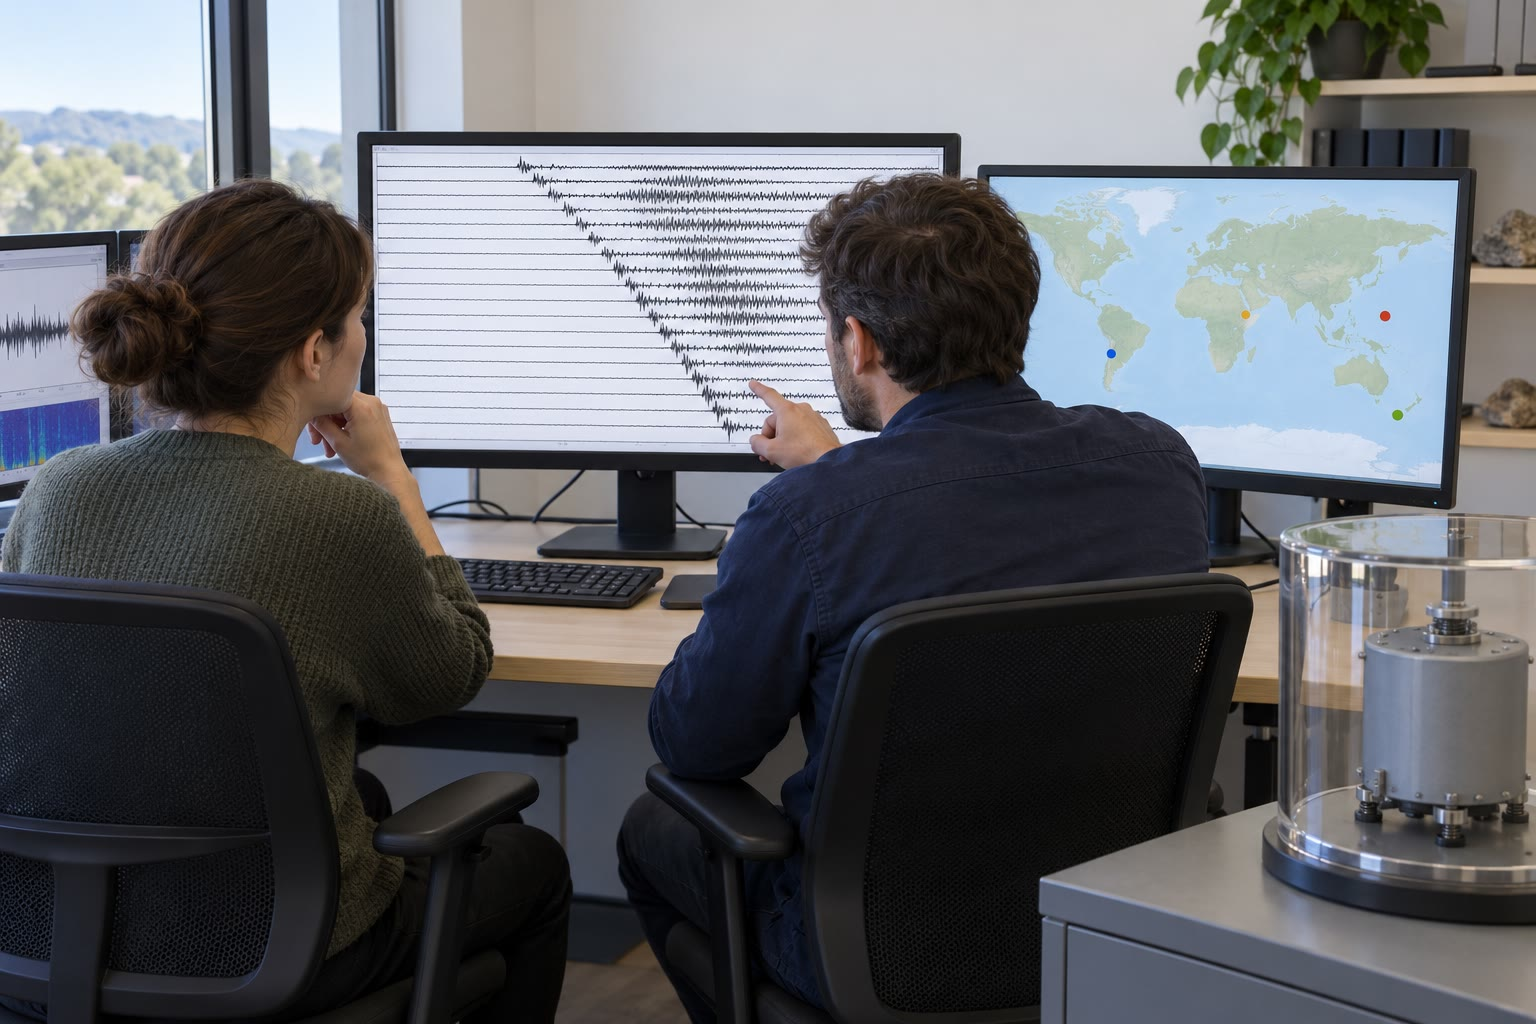
\includegraphics[width=\linewidth]{images/book3/ai/b1-seismic-analysis.jpg}

{\scriptsize Seismologists reading a record section, the traces of one
earthquake at stations sorted by distance (AI illustration).}
\end{minipage}
\end{inthelab}
% ledger: yvo:beachball

\section{Measuring the loading: geodesy}\label{sec:b1:earthquake-source:geodesy}

Between earthquakes, a locked fault is invisible to seismometers, but the
ground around it moves. Permanent satellite-positioning stations measure that
motion, and the way their velocities change across a fault tells how deep it
is locked.

\begin{definition}[Locking depth]\label{def:b1:earthquake-source:locking-depth}
The \emph{locking depth}\index{locking depth} of a fault is the depth down to
which it is locked between earthquakes, the fault below sliding steadily at the
long-term rate; it is the depth of the part of the fault that slips in the next
earthquake.
\end{definition}
% ledger: usgs:pp1515-thatcher

\begin{proposition}[Interseismic velocity across a strike-slip fault]\label{prop:b1:earthquake-source:interseismic}
Let a vertical \omterm{def:b1:faults-folds-fabrics:fault-types}{strike-slip fault} in an elastic half-space be locked from the
surface to the depth $D$, and slide at the rate $V$ below it. The velocity of
the surface parallel to the fault, at the distance $x$ from it, is
\[
  v(x) = \frac{V}{\pi}\arctan\frac{x}{D} .
\]
If the fault then slips by $s$ from the surface to the depth $D$ in an
earthquake, the surface moves by $u(x) = (s/\pi)\arctan(D/x)$ for $x > 0$, and by
$-u(-x)$ for $x < 0$.
\end{proposition}
\admitted

This model, due to Savage and Burford, is the simplest form of the \omterm{def:b1:earthquake-source:seismic-cycle}{elastic
rebound}, and the curve of the fence of the first figure. Its properties follow
from the formula.

\begin{proposition}[Reading the interseismic profile]\label{prop:b1:earthquake-source:profile}
In the model of \cref{prop:b1:earthquake-source:interseismic}:
\begin{enumerate}[label=(\alph*)]
  \item far from the fault the velocity tends to $\pm V/2$, the two plates
        moving at $V$ relative to each other;
  \item half of the change of velocity across the fault happens within the
        distance $D$ of it: $v(\pm D) = \pm V/4$;
  \item the shear-strain rate of the surface, $\mathrm dv/\mathrm dx$, is
        largest on the fault, where it equals $V/(\pi D)$;
  \item if the fault, after loading for the time $t$, slips by $s = Vt$ in an
        earthquake, the ground ends up displaced by $\pm s/2$ everywhere on
        either side: the cycle leaves no permanent bending, only the offset $s$
        on the fault.
\end{enumerate}
\end{proposition}

\begin{proof}
(a) $\arctan(x/D) \to \pm\pi/2$ as $x \to \pm\infty$. (b) $\arctan 1 = \pi/4$,
so $v(D) = V/4$, and $v$ is odd. (c) $\mathrm dv/\mathrm dx = (V/\pi D)/(1 +
x^2/D^2)$, largest at $x = 0$. (d) For $x > 0$, the loading has moved the
ground by $t\,v(x) = (s/\pi)\arctan(x/D)$ and the earthquake by
$(s/\pi)\arctan(D/x)$; since $\arctan y + \arctan(1/y) = \pi/2$ for $y > 0$,
the sum is $s/2$. The same holds with the signs reversed for $x < 0$.
\end{proof}

Property (b) gives the \omterm{def:b1:earthquake-source:locking-depth}{locking depth} from a profile of stations: it is the
distance from the fault at which the velocity has changed by a quarter of $V$
from its value on the fault. A shallow lock concentrates the strain near the
fault (the figure below), a deep one spreads it over a wide belt. Along the San
Andreas system, the \omterm{def:b1:earthquake-source:locking-depth}{locking depths} found from geodesy range from nearly 0, on
creeping segments, to \qty{26}{km}, and agree with the depths of the
earthquakes: the locked part is the \omterm{def:b1:stress-strain-rheology:strength-envelope}{seismogenic layer} of
\cref{ch:b1:stress-strain-rheology}. For a slip rate of
\qty{34}{mm.yr^{-1}} and a \omterm{def:b1:earthquake-source:locking-depth}{locking depth} of \qty{15}{km}, the shear-strain rate
on the fault is $\num{0.034}/(\pi\times\num{15000}) = \num{7.2e-7}$ per year,
which bends a line across the fault by less than a millimetre per kilometre in
a year, yet stores, over two centuries, the several metres of slip of a great
earthquake.
% ledger: sk:mu-locking, usgs:pp1515-wallace, usgs:pp1515-thatcher

\begin{omfigure}
\begin{tikzpicture}[font=\small]
\begin{axis}[omrecord, width=11cm, height=5.6cm, xmin=-100, xmax=100, ymin=-19, ymax=19,
    xlabel={distance from the fault $x$ (km)}, ylabel={velocity $v$ (\unit{mm.yr^{-1}})},
    legend style={font=\scriptsize, at={(0.02,0.96)}, anchor=north west}, legend cell align=left]
  \addplot[omDef, line width=0.9pt, dashed] table[x=x, y=v5] {figdata/out/bachelor-1-interseismic-profiles.dat};
  \addplot[omThm, line width=1.1pt] table[x=x, y=v15] {figdata/out/bachelor-1-interseismic-profiles.dat};
  \addplot[omProp, line width=0.9pt, dotted] table[x=x, y=v25] {figdata/out/bachelor-1-interseismic-profiles.dat};
  \legend{$D = \qty{5}{km}$, $D = \qty{15}{km}$, $D = \qty{25}{km}$}
  \draw[black!50, dashed] (axis cs:-100,17) -- (axis cs:100,17);
  \draw[black!50, dashed] (axis cs:-100,-17) -- (axis cs:100,-17);
  \node[anchor=north west, font=\scriptsize] at (axis cs:-30,17) {$+V/2$};
  \node[anchor=south west, font=\scriptsize] at (axis cs:30,-17) {$-V/2$};
  \draw[black!60] (axis cs:0,-19) -- (axis cs:0,19);
  \node[anchor=east, font=\scriptsize] at (axis cs:-1,5) {fault};
\end{axis}
\end{tikzpicture}
\par\smallskip{\small Velocity of the ground parallel to a locked \omterm{def:b1:faults-folds-fabrics:fault-types}{strike-slip
fault}, relative to the fault trace, for a slip rate $V = \qty{34}{mm.yr^{-1}}$,
that of the San Andreas fault at Wallace Creek, and three \omterm{def:b1:earthquake-source:locking-depth}{locking depths}
(\cref{prop:b1:earthquake-source:interseismic}). The shallower the lock, the
narrower the belt in which the velocity changes.}
\label{fig:b1:earthquake-source:interseismic}
\end{omfigure}
% ledger: usgs:pp1515-wallace

Satellite positioning measures the ground at a few stations. Radar satellites
measure it everywhere: two radar images of the same area taken from the same
orbit at different times are compared wave by wave, and the difference of
phase maps the change of the distance between the ground and the satellite,
point by point, a hundred metres apart, with no network of stations set up in
advance. The first such map, of a large Californian earthquake in 1992, showed
its coseismic displacement in a single picture and agreed with the slip
measured in the field and by surveying; the technique, radar interferometry,
belongs to the Year~3 volume.
% ledger: massonnet:1993

\section{How often: the Gutenberg--Richter law}\label{sec:b1:earthquake-source:gr}

Small earthquakes are far more common than large ones, and in a remarkably
regular way.

\begin{proposition}[Gutenberg--Richter law]\label{prop:b1:earthquake-source:gutenberg-richter}
In a region and a period\index{Gutenberg--Richter law}, the number $N$ of earthquakes of magnitude at least
$M$ follows
\[
  \log_{10} N = a - bM ,
\]
for every $M$ above the \omterm{def:b1:earthquake-source:b-value}{magnitude of completeness} of the catalogue, with
constants $a$ and $b$ that depend on the region; $b$ is close to 1 in most
active regions.
\end{proposition}
\admitted
% ledger: fd:1993, gr:1944

The law is a result of observation, published by Beno Gutenberg and Charles
Richter for California in 1944 and since found everywhere; no theory yet
derives it, nor the value of $b$.
% ledger: gr:1944

\begin{definition}[b-value, magnitude of completeness]\label{def:b1:earthquake-source:b-value}
The constant $b$ of the \omterm{prop:b1:earthquake-source:gutenberg-richter}{Gutenberg--Richter law} of a region is its
\emph{b-value}\index{b-value}. The \emph{magnitude of
completeness}\index{magnitude of completeness} of a catalogue is the smallest
magnitude above which it records every earthquake of the region and period.
\end{definition}

A \omterm{def:b1:earthquake-source:b-value}{b-value} of 1 means ten times fewer earthquakes for each unit of magnitude.
Below the \omterm{def:b1:earthquake-source:b-value}{magnitude of completeness}, the counts fall short of the line, because
small earthquakes are recorded by too few stations to be located: the law
seems to bend, and $b$ must be measured above it. For the whole Earth,
divided into shallow, intermediate and deep earthquakes, the measured values
lie between 0.72 and 1.34, but they differ by \qty{30}{\percent} or more from
one catalogue, range of magnitude or method to another: a value far from 1 is
first a reason to check the catalogue.
% ledger: fd:1993

\begin{omfigure}
\begin{tikzpicture}[font=\small]
\begin{axis}[omrecord, width=6.4cm, height=5.8cm, ymode=log, xmin=5.8, xmax=9.3, ymin=0.01, ymax=300,
    xlabel={magnitude $M$}, ylabel={events of magnitude $\ge M$ per year},
    log basis y=10, title={(a) frequency and magnitude}, title style={font=\small}]
  \addplot[omProp, line width=0.9pt, domain=5.8:9.3] table[x=M, y=rate] {figdata/out/bachelor-1-gutenberg_richter-fit.dat};
  \addplot[only marks, mark=*, mark size=1.3pt, omDef] table[x=M, y=rate] {figdata/out/bachelor-1-gutenberg_richter-counts.dat};
  \draw[black!50, dashed] (axis cs:7.5,0.01) -- (axis cs:7.5,300);
  \node[anchor=south west, font=\scriptsize, omProp] at (axis cs:8.45,0.5) {$b = 1.01$};
  \node[anchor=north west, font=\scriptsize, align=left] at (axis cs:7.55,200) {fitted over\\ $6.0 \le M \le 7.5$};
\end{axis}
\begin{axis}[omrecord, at={(7.6cm,0)}, width=6.4cm, height=5.8cm, xmin=5.8, xmax=9.3, ymin=0, ymax=1.05,
    xlabel={magnitude $M$}, ylabel={share of the moment from events $\ge M$},
    title={(b) where the moment goes}, title style={font=\small}]
  \addplot[const plot, omDef, line width=0.9pt] table[x=M, y=share] {figdata/out/bachelor-1-gutenberg_richter-moment.dat};
\end{axis}
\end{tikzpicture}
\par\smallskip{\small The \num{7031} earthquakes of magnitude 6 or more in the
world, 1976--2025 (U.S. Geological Survey catalogue). (a) The yearly number of
earthquakes of magnitude at least $M$; the line is the least-squares fit of
$\log_{10} N$ against $M$ from 6.0 to 7.5, where each count exceeds 200:
$\log_{10} N = 8.20 - 1.01\,M$ per year. Above magnitude 8 the few events fall
below the line. (b) The share of the total \omterm{def:b1:earthquake-source:moment}{seismic moment} released by the
earthquakes of magnitude at least $M$, each moment computed as
$10^{1.5M + 9.1}$\,\unit{N.m}: the 40 earthquakes of magnitude 8 or more
released \qty{63}{\percent} of it.}
\label{fig:b1:earthquake-source:gutenberg-richter}
\end{omfigure}
% ledger: data:usgs-comcat (fit and shares computed in figdata/bachelor-1/gutenberg_richter.py)

For the world catalogue of the figure, the law with $a = 8.20$ and $b = 1.01$
predicts 14 earthquakes of magnitude 7 or more a year, as observed, and 1.35 of
magnitude 8 or more, while 40 in fifty years, 0.8 a year, were recorded. Whether
the largest earthquakes are truly fewer than the line, as the finite size of
faults would suggest, or only rare enough to be missing from fifty years, is not
settled by so few events. About one magnitude in nine in this catalogue is a
surface-wave or body-wave magnitude, which saturate; the largest events all
have \omterm{def:b1:earthquake-source:mw}{moment magnitudes}.
% ledger: data:usgs-comcat

The many small earthquakes do little of the work. Their number grows ten times
for each unit of magnitude less, but their moments shrink 31.6 times.

\begin{proposition}[The largest earthquakes release most of the moment]\label{prop:b1:earthquake-source:largest}
Let earthquakes follow the \omterm{prop:b1:earthquake-source:gutenberg-richter}{Gutenberg--Richter law} with $b < 1.5$, up to a
largest magnitude $M_{\max}$, and let them be grouped in bins one unit of
magnitude wide, the top bin ending at $M_{\max}$. Then the earthquakes of the top
bin release more than the fraction $1 - 10^{-(1.5 - b)}$ of the total moment,
however small the smallest magnitude counted: more than \qty{68}{\percent} for
$b = 1$.
\end{proposition}

\begin{proof}
Let the bins be numbered $k = 0, 1, \dots, K$ from the smallest, the bin $k$
running from $M_k$ to $M_k + 1$, with $M_{k+1} = M_k + 1$. By the law, the number
of earthquakes in bin $k$ is $10^{a - bM_k} - 10^{a - b(M_k+1)} =
10^{a - bM_k}(1 - 10^{-b})$; by \cref{prop:b1:earthquake-source:moment-steps}
the moment of each lies between $10^{1.5M_k + 9.1}$ and $10^{1.5}$ times that,
and since every bin is the previous one shifted by one unit, the moment of
bin $k$ is $C q^k$ for a constant $C$ and the ratio
$q = 10^{-b}\times10^{1.5} = 10^{1.5 - b} > 1$. The total is the geometric sum
\[
  S = C(1 + q + \dots + q^K) = C\,\frac{q^{K+1} - 1}{q - 1} ,
\]
and the share of the top bin is
\[
  \frac{C q^K}{S} = \frac{q^K (q - 1)}{q^{K+1} - 1}
  > \frac{q^K (q - 1)}{q^{K+1}} = 1 - \frac1q = 1 - 10^{-(1.5 - b)} .
\]
For $b = 1$, $1 - 10^{-0.5} = 0.684$.
\end{proof}

In the world catalogue the share is of this order: the top unit of magnitude,
from 8.1 to 9.1, released over half of the moment of fifty years, and the two
largest earthquakes, Sumatra--Andaman in 2004 and Tohoku in 2011, with
magnitudes of 9.1, released \qty{29}{\percent} of it by themselves. The moment a
plate boundary must release is set by its slip rate; the proposition says that
it is released almost entirely in its largest earthquakes, and that the many
small ones, however frequent, do not relieve a fault of the next great one.
% ledger: data:usgs-comcat, usgs:sumatra-mt, usgs:tohoku-mt

\section{Exercises}

\begin{exercise}[$\star$]\label{exo:b1:earthquake-source:1}
(a) Compute the \omterm{def:b1:earthquake-source:mw}{moment magnitude} of an earthquake of \omterm{def:b1:earthquake-source:moment}{seismic moment}
\qty{4e17}{N.m}. (b) The Tohoku earthquake had $M_0 = \qty{5.59e22}{N.m}$:
check its magnitude. (c) What \omterm{def:b1:earthquake-source:moment}{seismic moment} has an earthquake of magnitude
7.0?
% ledger: usgs:tohoku-mt
\end{exercise}

\begin{exercise}[$\star$]\label{exo:b1:earthquake-source:2}
A \omterm{def:b1:faults-folds-fabrics:fault-types}{strike-slip fault} is loaded at \qty{25}{mm.yr^{-1}}, and its earthquakes
each slip by about \qty{3}{m}. (a) What is their \omterm{def:b1:earthquake-source:seismic-cycle}{recurrence interval} if the
fault is fully locked between them? (b) And if half the slip rate is taken up
by steady creep?
\end{exercise}

\begin{exercise}[$\star$]\label{exo:b1:earthquake-source:3}
How many times larger is the \omterm{def:b1:earthquake-source:moment}{seismic moment} of an earthquake of magnitude 7.4
than that of an earthquake of magnitude 6.2? How many earthquakes of magnitude
6.2 would release the same moment?
\end{exercise}

\begin{exercise}[$\star$]\label{exo:b1:earthquake-source:4}
In a region with $b = 1$, a thousand earthquakes of magnitude 3 or more are
recorded each year. How many of magnitude 5 or more, and of magnitude 6 or
more, are expected each year? What is the mean time between earthquakes of
magnitude 7 or more?
\end{exercise}

\begin{exercise}[$\star\star$]\label{exo:b1:earthquake-source:5}
The 1906 earthquake broke the San Andreas fault over about \qty{430}{km}.
(a) Assuming the rupture reached \qty{15}{km} deep with an average slip of
\qty{4}{m}, and $\mu = \qty{30}{GPa}$, compute its \omterm{def:b1:earthquake-source:moment}{seismic moment} and \omterm{def:b1:earthquake-source:mw}{moment
magnitude}. (b) How much does the magnitude change if the rupture was only
\qty{10}{km} deep? (c) Which of the two estimates is closer to 7.9?
% ledger: pp1515:1906, usgs:hist-mw
\end{exercise}

\begin{exercise}[$\star\star$]\label{exo:b1:earthquake-source:6}
The rupture of the Tohoku earthquake was about \qty{400}{km} long and
\qty{150}{km} wide, and its moment \qty{5.59e22}{N.m}. (a) Compute its
average slip with $\mu = \qty{30}{GPa}$. (b) The Pacific plate sinks beneath
Japan at about \qty{83}{mm.yr^{-1}}: how long does it take to accumulate this
slip if the interface is fully locked? (c) And if the locked fraction is 0.8,
or 0.5?
% ledger: usgs:tohoku-mt, usgs:tohoku-summary
\end{exercise}

\begin{exercise}[$\star\star$]\label{exo:b1:earthquake-source:7}
One \omterm{def:b1:earthquake-source:focal-mechanism}{nodal plane} of the 2004 Sumatra--Andaman earthquake has \omterm{def:b1:geological-maps:attitude}{strike} $329$, \omterm{def:b1:geological-maps:attitude}{dip}
\ang{8} and \omterm{def:b1:faults-folds-fabrics:fault-elements}{rake} \ang{110}. (a) Write $\mathbf n$ and $\mathbf d$ in east, north
and up components. (b) Find the \omterm{def:b1:geological-maps:attitude}{strike}, \omterm{def:b1:geological-maps:attitude}{dip} and \omterm{def:b1:faults-folds-fabrics:fault-elements}{rake} of the \omterm{def:b1:earthquake-source:focal-mechanism}{auxiliary plane}.
(c) Find the \omterm{def:b1:field-lab-methods-1:trend-plunge}{trends} and \omterm{def:b1:field-lab-methods-1:trend-plunge}{plunges} of the P and T axes. (d) Which plane is the
fault, and what kind of fault is it?
% ledger: usgs:sumatra-mt
\end{exercise}

\begin{exercise}[$\star\star$]\label{exo:b1:earthquake-source:8}
A vertical fault striking $045$ slips \omterm{def:b1:faults-folds-fabrics:fault-types}{dextrally}. (a) For waves leaving the focus
horizontally toward stations due north, east, south and west, which arrive as
pushes and which as pulls? (b) Give the \omterm{def:b1:field-lab-methods-1:trend-plunge}{trends} of the P and T axes. (c) Show
that a \omterm{def:b1:faults-folds-fabrics:fault-types}{sinistral} slip on a vertical plane striking $135$ gives the same \omterm{def:b1:earthquake-source:focal-mechanism}{first
motions}.
\end{exercise}

\begin{exercise}[$\star\star$]\label{exo:b1:earthquake-source:9}
Across a locked \omterm{def:b1:faults-folds-fabrics:fault-types}{strike-slip fault}, the far-field stations on the two sides move
at \qty{40}{mm.yr^{-1}} relative to each other. A station \qty{10}{km} from the
fault moves at \qty{10}{mm.yr^{-1}} relative to the fault trace. (a) Find the
\omterm{def:b1:earthquake-source:locking-depth}{locking depth}. (b) Predict the velocity of a station \qty{30}{km} from the
fault. (c) Compute the shear-strain rate on the fault.
\end{exercise}

\begin{exercise}[$\star\star\star$]\label{exo:b1:earthquake-source:10}
(a) Show that, if $b$ were larger than 1.5, the total moment of the earthquakes
of a region would be dominated by the smallest ones. (b) What share of the
moment does the top unit of magnitude release at least, for $b = 0.8$? (c) With
the world catalogue's $a = 8.20$ and $b = 1.01$ per year, how many earthquakes of
magnitude 9 or more would the law predict in fifty years? The catalogue of
1976--2025 holds two; comment.
% ledger: data:usgs-comcat
\end{exercise}

\begin{exercise}[$\star\star\star$]\label{exo:b1:earthquake-source:11}
A straight fence is built across a locked \omterm{def:b1:faults-folds-fabrics:fault-types}{dextral} fault with $V =
\qty{34}{mm.yr^{-1}}$ and $D = \qty{15}{km}$. (a) After 150 years, by how much
have the posts \qty{1}{km}, \qty{15}{km} and \qty{50}{km} east of the fault
moved along it, relative to the post on the fault? (b) The fault then slips by
the whole deficit in an earthquake. What is the slip, and how far does each of
the three posts move during the earthquake? (c) Check part (d) of
\cref{prop:b1:earthquake-source:profile} on the three posts.
% ledger: usgs:pp1515-wallace
\end{exercise}

\begin{exercise}[$\star\star\star$]\label{exo:b1:earthquake-source:12}
An earthquake has a horizontal \omterm{def:b1:earthquake-source:focal-mechanism}{P axis} trending $000$ and a horizontal \omterm{def:b1:earthquake-source:focal-mechanism}{T axis}
trending $090$. (a) Show that its \omterm{def:b1:earthquake-source:focal-mechanism}{nodal planes} are vertical and \omterm{def:b1:geological-maps:attitude}{strike} $045$
and $135$, using $\mathbf n$, $\mathbf d = (\mathbf T \pm \mathbf P)/\sqrt2$.
(b) Give the sense of slip on each plane. (c) If the fault had formed as a new
fault in a rock with $\phi = \ang{30}$, under a $\sigma_1$ along the \omterm{def:b1:earthquake-source:focal-mechanism}{P axis},
at what \omterm{def:b1:geological-maps:attitude}{strikes} would it lie, and why is the \omterm{def:b1:earthquake-source:focal-mechanism}{P axis} only an approximation of
$\sigma_1$? (d) A mapped fault nearby \omterm{def:b1:geological-maps:attitude}{strikes} $040$. Which \omterm{def:b1:earthquake-source:focal-mechanism}{nodal plane} is
likely the fault, and what is its sense of slip?
\end{exercise}

\section{Problem: The next great earthquake on a locked fault}

\begin{problem}[{Weekend problem --- a locked segment of a strike-slip plate
boundary, from its loading and its past earthquakes to the magnitude of the
next}]
\label{pb:b1:earthquake-source:1}
% values: calc/ch18.py; an invented fault (the numbers are of a realistic order)
A straight, vertical \omterm{def:b1:faults-folds-fabrics:fault-types}{strike-slip fault} forms the boundary between two plates.
One segment of it, \qty{250}{km} long, is locked; its earthquakes start no
deeper than \qty{15}{km}. Trenches dug across it date its last four great
earthquakes to about 1050, 1290, 1480 and 1712, with offsets of \num{7.0},
\num{6.0}, \num{5.5} and \qty{7.5}{m}. Permanent stations far from the fault on
the two sides move at \qty{30}{mm.yr^{-1}} relative to each other. Take $\mu =
\qty{30}{GPa}$, the year 2025 as the present, and give magnitudes to 0.01.

\medskip
\noindent\textbf{Part I --- The loading.}
\begin{enumerate}
  \item Compute the intervals between the four earthquakes and their mean.
  \item Compute the mean offset, and the \omterm{def:b1:earthquake-source:seismic-cycle}{recurrence interval} it implies with
        \cref{prop:b1:earthquake-source:recurrence} for a fully locked fault.
  \item Compute the slip rate implied by the trench alone, from the offsets of
        the last three earthquakes and the time between the first and the last.
        Compare with the geodetic rate.
  \item How long ago was the last earthquake, and what slip deficit has
        accumulated since, if the segment is fully locked?
  \item Compare this deficit with the offsets in the trench. Is the next
        earthquake overdue?
  \item Why can the trench not give the date of the next one?
\end{enumerate}

\medskip
\noindent\textbf{Part II --- The size of the next earthquake.}
\begin{enumerate}[resume]
  \item What is the area of the locked part of the segment?
  \item Compute the \omterm{def:b1:earthquake-source:moment}{seismic moment} of an earthquake that would release the
        whole deficit.
  \item Compute the \omterm{def:b1:earthquake-source:mw}{moment magnitude} of the 1712 earthquake, assuming it broke
        the same area with its trench offset as average slip.
  \item By what factor does the moment of the next earthquake exceed that of
        1712, and how many units of magnitude is that?
  \item If only half of the segment broke, with the same slip, what would the
        magnitude be?
  \item Give the \omterm{def:b1:earthquake-source:moment}{seismic moment} that the segment accumulates each year.
\end{enumerate}

\medskip
\noindent\textbf{Part III --- Frequency and energy.}
\begin{enumerate}[resume]
  \item The regional catalogue follows $\log_{10} N = 4.3 - M$ per year, from
        all the faults of the region. What is its \omterm{def:b1:earthquake-source:b-value}{b-value}, and how many
        earthquakes of magnitude 5 or more, and 6 or more, does it give each
        year?
  \item What mean time between earthquakes of magnitude 7 or more does it give,
        and of magnitude 8 or more?
  \item Compare the recurrence of a great earthquake from the catalogue with
        the one from the trench. What does the difference say about using the
        law of small earthquakes to forecast great ones?
  \item The earthquakes of magnitude 5 to 8 of the regional law release, all
        together, about \qty{5.5e17}{N.m} a year. What fraction of the moment
        of the segment is that?
  \item How many times more energy than an earthquake of magnitude 6 would
        the next great earthquake radiate?
  \item Using \cref{prop:b1:earthquake-source:largest}, explain why the
        moderate earthquakes of the segment do not relieve it.
\end{enumerate}

\medskip
\noindent\textbf{Part IV --- The locking depth from the stations.}
\begin{enumerate}[resume]
  \item A profile of stations across the segment gives, relative to the fault
        trace, the velocities $-11.6$, $-7.5$, $-3.1$, $3.1$, $7.5$ and
        \qty{11.6}{mm.yr^{-1}} at $x = -40$, $-15$, $-5$, $5$, $15$ and
        \qty{40}{km}. Check that the profile is antisymmetric, and give the
        velocities expected far from the fault.
  \item From the station at \qty{15}{km}, compute the \omterm{def:b1:earthquake-source:locking-depth}{locking depth}.
  \item Compute it again from the stations at \qty{5}{km} and \qty{40}{km}, and
        explain the small differences.
  \item Compare the \omterm{def:b1:earthquake-source:locking-depth}{locking depth} with the depth of the earthquakes, and say
        why they should agree.
  \item Compute the shear-strain rate on the fault.
  \item To 0.01, what is the \omterm{def:b1:earthquake-source:mw}{moment magnitude} of the earthquake that would
        release the whole slip deficit of the segment?
\end{enumerate}
\end{problem}
